\section{Usages}
An important feature of XML Encryption is that it can be used directly in XML\@.
Which makes it possible to encrypt just some elements or some content of
elements instead of the full XML file. Encrypting arbitrary data is also
supported however.
\section{EncryptedData}
\section{Examples}
\begin{minted}{xml}
  <?xml version='1.0'?>
  <PaymentInfo xmlns='http://example.org/paymentv2'>
    <Name>John Smith</Name>
    <CreditCard Limit='5,000' Currency='USD'>
      <Number>4019 2445 0277 5567</Number>
      <Issuer>Example Bank</Issuer>
      <Expiration>04/02</Expiration>
    </CreditCard>
  </PaymentInfo>
\end{minted}
\section{Encryption Algorithms}
\subsection{Symmetric}
\begin{minted}{xml}
    <EncryptedData xmlns='http://www.w3.org/2001/04/xmlenc#'
        Type='http://www.w3.org/2001/04/xmlenc#Element'/>
  [s2]   <EncryptionMethod
          Algorithm='http://www.w3.org/2001/04/xmlenc#tripledes-cbc'/>
         <ds:KeyInfo xmlns:ds='http://www.w3.org/2000/09/xmldsig#'>
  [s4]     <ds:KeyName>John Smith</ds:KeyName>
         </ds:KeyInfo>
  [s6]   <CipherData><CipherValue>DEADBEEF</CipherValue></CipherData>
       </EncryptedData>
\end{minted}

\begin{table}
    \begin{tabulary}{\textwidth}{cL}
        \toprule
        Label & Explanation \\
        \midrule
        s2 & This (3DES CBC) is a symmetric key cipher. \\

        s4 & The symmetric key has an associated name “John Smith”. \\

        s6 & CipherData contains a CipherValue, which is a base64 encoded octet
        sequence. Alternately, it could contain a CipherReference, which is a
        URI reference along with transforms necessary to obtain the encrypted
        data as an octet sequence. \\
        \bottomrule
    \end{tabulary}
    \caption{Explanation}
\end{table}

\subsection{Asymmetric}
Asymmetric encryption (or public key cryptography) uses two keys instead of one

\begin{enumerate}
    \item The private key typically is used to encrypt the message
    \item The public key is used to decrypt the message
\end{enumerate}
See Figure~\ref{fig:public_key} for a simple explanatory image.

\begin{figure}
    \center{}
    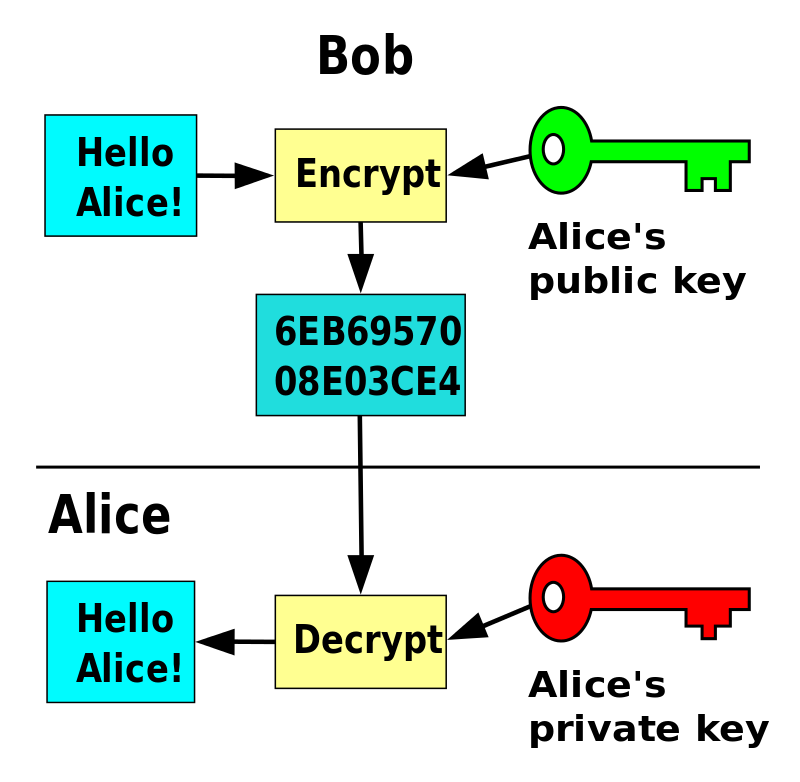
\includegraphics[width=0.5\textwidth]{public_key}
    \caption{Bob encrypts his message with Alice's public
    key}\label{fig:public_key}
\end{figure}

